\nextslide{Le v\'erificateur de bytecode}
%\includegraphics[width=\linewidth]{java2.ps}\\

Bas\'e sur l'algorithme de {\purple Kildall}:\\ 
A chaque instruction $i$, on associe un \'etat de typage $St$, 
une abstraction de l'\'etat de la VM $S$.\\
En it\'erant sur les instructions,
\blist 
\item On calcule l'\'etat de typage $St_{\textrm{exec}}$
obtenu apr\`es l'ex\'ecution de l'instruction.  $St_{\textrm{exec}} = \textrm{exec}(i,St)$
\item On unifie  $St_{\textrm{exec}}$ avec les \'etats de typage des
 successeurs. $St_{\textrm{succ}(i)}'$ = $St_{\textrm{succ}(i)} \cup St_{\textrm{exec}}$
\item Quand les \'etats ne changent plus, l'algorithme se termine
\elist


\nextslide{Propri\'et\'es \`a d\'emontrer}
%Propri\'et\'es simples: % (d\'emontrable {\purple automatiquement}):
\blist
\item  Les d\'ebordements arithm\'etiques et les renvois d'exception

%\elist\norm
%Propri\'et\'es non triviales: %(en g\'en\'eral d\'emontrable seulement
%{\purple interactivement}):
%\blist\small
\item Terminaison:
%$\forall$ i: Instruction,  
$St_{succ(i)}$ $\leq$ $exec(i, St_{i}) \cup St_{succ(i)}$
\item Correction:
\begin{center}\begin{minipage}{8cm} 
$$
\begin{array}{rcl}
{\purple St_{i}} &  
{\purple \xrightarrow[]{\textrm{\ \ \ \ \ exec\ \ \ \ \ }}} & 
{\purple St_{\textrm{succ}(i)} = \textrm{exec}(i, St_{i}) \cup St_{\textrm{succ}(i)}} \\ 
\uparrow &  & \uparrow \\
S_{i} & \xrightarrow[\ \ \ \ \ {\textrm eval}\ \ \ \ \ ]{} & S_{\textrm{succ}(i)}\\
\end{array}$$
\end{minipage}
\end{center}

%\includegraphics[width=0.2\linewidth]{commut.ps}\\
\elist

\nextslide{Architecture Choisie}
4 classes principales:
\blist
\item VerificationException
\item State
\item Instruction
\item Verifier
\elist \small
Les classes State et Instruction sont ensuites raffin\'ees pour
 correspondre \`a une machine virtuelle Java, les 
classes Verifier et VerificationException n'ont plus \`a \^etre modifi\'ees.

\nextslide{Quelques statistiques}
\small
\begin{tabular}{p{0.34\textwidth} c c c c}
{\bf Classes:} & VerificationException & State & Instruction & Verifier \\
\raggedright {\bf Lignes de code:} & 13 & 14 & 47 & {\purple 66}\\
\raggedright {\bf Lignes d'annotations:} & 5 & 20 & 54 & {\purple 81}\\
\raggedright {\bf Nbr. d'OPs :} &  60 & 26 & 129 & {\purple 627} \\
\raggedright {\bf Simplify:} &  60 & 26 & 53 & {\purple 5}\\


\end{tabular}